\section{Schedules}

  We have two pipelines, the \textbf{\textit{catalogue}} pipeline that is responsible for all the data that is currently accessible to partners on iPlayer
  and the new \textbf{\textit{schedules}} pipeline. We first have to ingest the schedule data from another source, which consists of over 1000 files and 
  then parse that data for what we want to share with partners. This parsed data is then stored in redis for future use. In the older catalogue pipeline 
  this process was done by an EC2 (server), however with this pipeline we wanted less to manage and decided to go with a lambda (serverless) approach. To speed 
  up ingestion of data we decided to experiment with multiple lambdas being invoked at the same time for concurrent processing of the files. 
  This is the part of the project I was tasked to document/create.
  
  \begin{figure}[H]
    \centering
    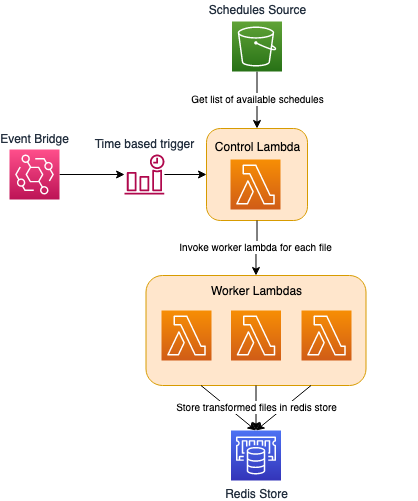
\includegraphics[width=6cm]{assets/ingester.drawio.png}
    \caption{Ingester AWS architecture.}
    \label{fig:ingesterArch}
  \end{figure}

  Figure 4 shows what the cloud infrastructure on AWS looks like. We get an event from event bridge, the available data is then retrieved from source and the
  parsing is then handed over to multiple concurrent lambdas. Finally this data is stored in redis for the next component in the pipeline to use. I have 
  illustrated this flow in the sequence diagram below.

  \begin{figure}[H]
    \centering
    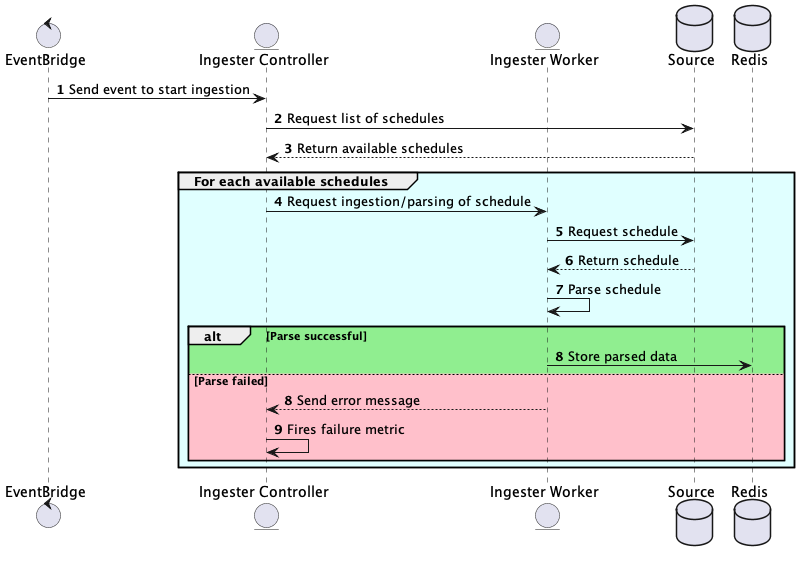
\includegraphics[width=8cm]{assets/diagrams/ingesterBasicFlow.png}
    \caption{Ingester basic execution sequence diagram.}
    \label{fig:ingesterFlow}
  \end{figure}

  For completeness I have also drawn a sequence diagram for the removal of old schedules from the redis store. This process is done just before the 
  parallelised lambdas are called to do their work. Removal is important here as if they were not removed it would have a knock on effect down the pipeline 
  as there would be unnecessary processing done for schedules that are no longer being used or accessible to partners.

  \begin{figure}[H]
    \centering
    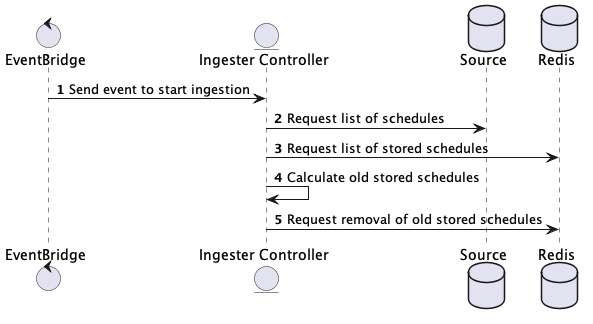
\includegraphics[width=8cm]{assets/diagrams/ingesterDataRemoval.png}
    \caption{Ingester old data removal sequence diagram.}
    \label{fig:ingesterScheduleRemoval}
  \end{figure}

  In the pipeline there is a second component called the \textit{Schedule Generator} that is responsible for outputting the data in a format partners will
  receive. For this component we did not have the worker lambda, and instead had a single lambda do all the processing. The two graphs belows show the 
  difference in lambda runtime between the two components.

  \begin{figure}[H]
    \centering
    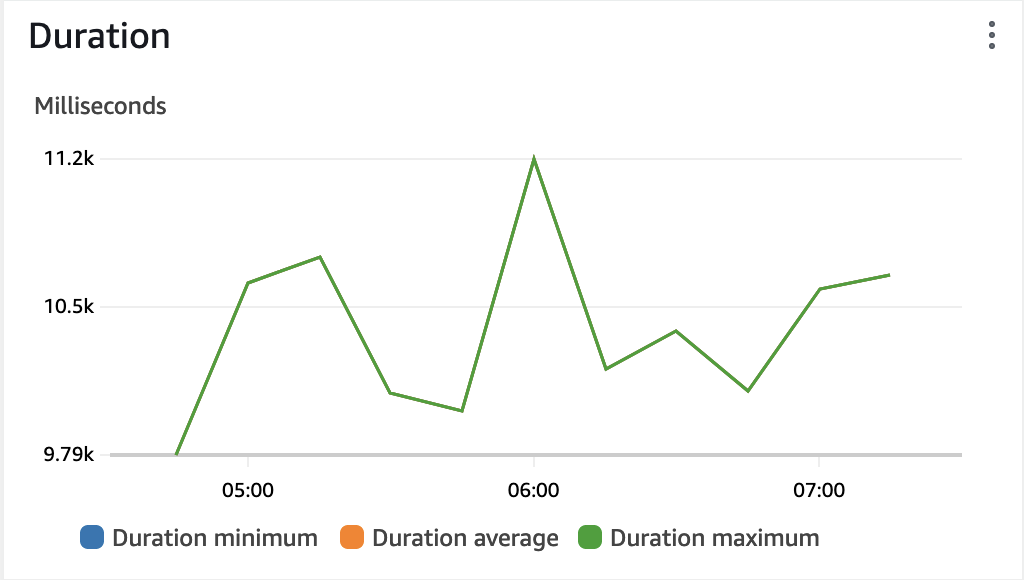
\includegraphics[width=6cm]{assets/ingesterDuration.png}
    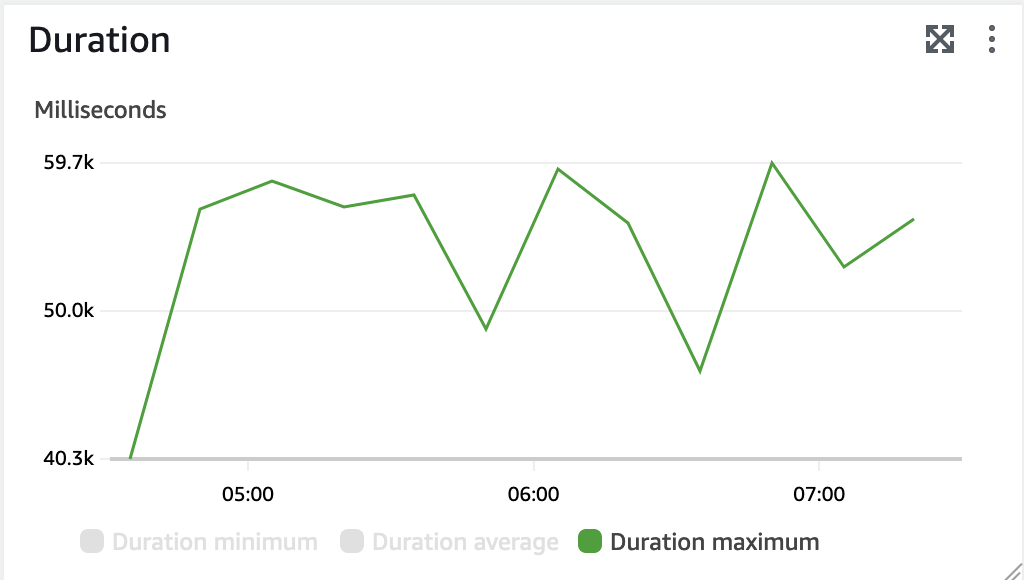
\includegraphics[width=6cm]{assets/generatorDuration.png}
    \caption{Screenshot of AWS lambda duration for schedule Ingester (left) and Generator (right).}
    \label{fig:lambdaDurationDifference}
  \end{figure}

  As can be seen, using parallelised lambdas is 4x quicker on average than using a single lambda. This is important as the quicker this pipeline can run
  the 'fresher' the data is for partners. After seeing these results there is now some talks about also changing the Schedule Generator to use the same 
  pattern.

  \vspace{0.2cm}

  This was also the first project where we upgraded to using the new version of the AWS SDK. This was something we hadn't looked into however was something
  that would be beneficial when we had to upgrade to node 18. AWS would no longer package version 2 of their SDK by default in lambdas. This would result in
  \todo[noline, size=\small]{L3, T2}
  an extra ~70MB of unpacked data being added to the final build which would slow down our build time and cost us a little bit more money, albeit fractions of
  a penny. I lead the investigation into using the new SDK and if it was feasible. This upgrade then also lead to the upgrade of our credentials provider
  which had security vulnerabilities that needed fixing.

  \begin{figure}[H]
    \centering
    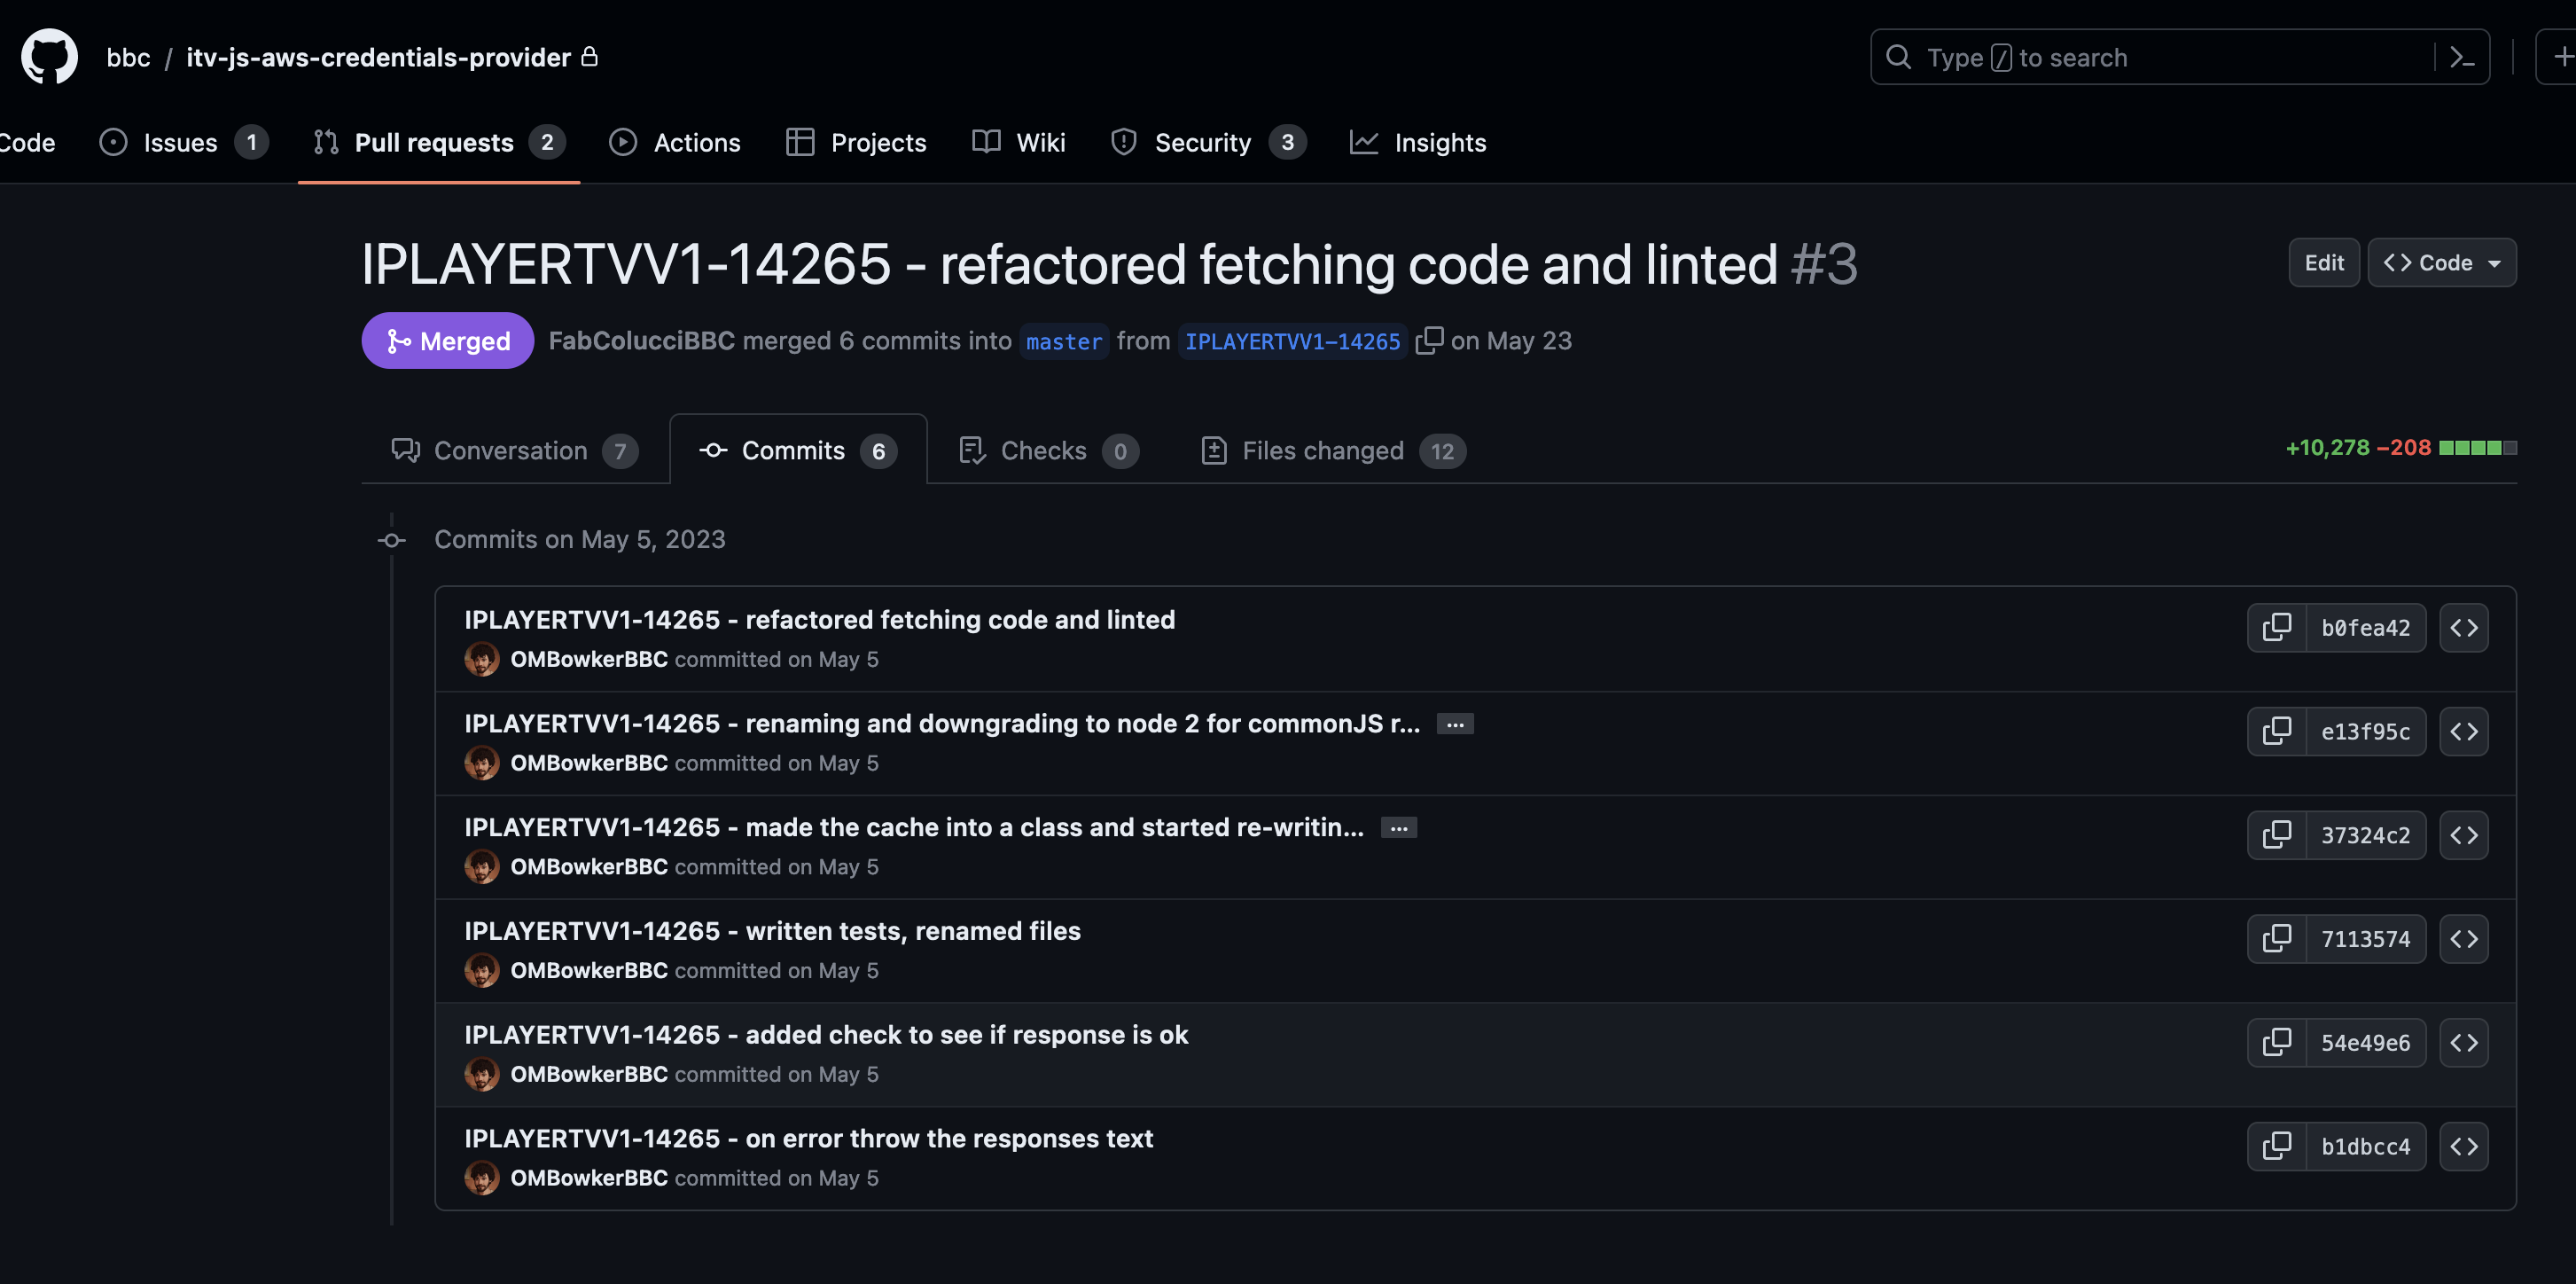
\includegraphics[width=6cm]{assets/credentialsRefactorCommits.png}
    \caption{Screenshot commits for credentials refactor.}
    \label{fig:credentialsRefactor}
  \end{figure}

  \newpage
